\chapter{Referencial teórico}
\label{cap:referencial-teorico}

  Neste capítulo esclarecemos os conceitos teóricos necessários para o
entendimento do trabalho e a metodologia proposta. Inicialmente, abordamos
aspectos da visualização de dados do tráfego, que abrange uma variedade de
cenários conforme os objetivos, tipos de dado e diferentes representações
visuais da informação. Neste contexto, destacamos o \emph{bundling}, uma
técnica bastante usada na visualização de grandes quantidades de dados do
tráfego. Apresentamos os detalhes da técnica e uma breve consideração sobre os
avanços recentes nesta área. Por fim, considerando que neste trabalho faremos o
uso de dados simulados do tráfego de veículos, apresentamos o simulador
InterSCSimulator.

\section{Visualização de dados do tráfego}

  A análise de dados do tráfego tem um histórico antigo. \citet{Chen2015} fazem
um levantamento de várias pesquisas de análise e visualização de dados do
tráfego de pessoas, carros e embarcações. Eles apresentam uma taxonomia
conforme algumas características observadas, como o objetivo da visualização,
formato dos dados do tráfego e formas de apresentação de suas propriedades.
Nesta seção apresentamos essa taxonomia, que é importante para um melhor
entendimento da área e dos esforços que têm sido feitos no campo da
visualização de dados do tráfego.

\subsection{Quanto ao Objetivo da Visualização}

  Segundo \citet{Chen2015}, os trabalhos e sistemas de software sobre análise e
visualização de dados do tráfego podem ser classificadas em quatro categorias
de acordo com seus objetivos e a tarefa a que servem.

\begin{description}
  \item[Monitoramento do tráfego:] esse tipo de aplicação
foca no monitoramento em tempo real para descobertas instantâneas de eventos no
tráfego, como câmeras de gravação ao vivo e sistemas de alerta.

  \item[Descoberta de padrões e clusterização:] para a descoberta de padrões e
tendências de mobilidade, algumas aplicações utilizam métodos para o
agrupamento visual de trajetórias ou novas abstrações dos dados.

  \item[Exploração e predição:] outras aplicações focam em fornecer mecanismos
de pesquisa e exploração dos dados para que os usuários investiguem os dados
que justifiquem situações do tráfego, como congestionamentos, ou ainda técnicas
de predição para prever essas situações (e.g. predizer que haverá
congestionamento devido a ocorrência de chuva).

  \item[Planejamento de rotas e recomendação:] sistemas de transporte
inteligentes contam essencialmente com recomendações de trajetos para usuários
do transporte, várias soluções existem com esse propósito, que podem envolver monitoramento
em tempo real ou análise histórica no processo de recomendação.
\end{description}

\subsection{Quanto ao Tipo de Coleta dos Dados}

  Dados do tráfego são tipicamente coletados a partir de sensores e dispositivos
eletrônicos. A estrutura desses conjuntos de dados dependem do modo de operação
dos sensores e dispositivos que registram a movimentação dos objetos. \citet{Chen2015}
os dividem em três classes:

\begin{description}
  \item[Baseado em pontos de interesse:] a posição de um objeto é gravada assim
que ele entra na área do sensor. Como uma câmera de vídeo que capta a
movimentação e orientação de um veículo assim que ele passa pela área de
monitoramento.

  \item[Baseado em ações:] as informações sobre um objeto podem estar associados
a certas atividades. O usuário de um aparelho celular por exemplo, tem sua
atividade e localização registrados pela rede GSM quando o mesmo efetua uma
chamada.

  \item[Baseado em sinais de dispositivos:] Um dispositivo de localização
carregado por um objeto constantemente grava e envia suas informações de
localização para uma central, como aparelhos de GPS instalados em um ônibus do
transporte público de uma cidade.  \end{description}

  Uma série de posições de localização ao longo do tempo formam a trajetória de
um objeto. Uma trajetória contém informações temporais, que permitem traçar uma
linha do tempo da movimentação, e informações espaciais, que contém a posição
em cada momento no tempo. A frequência de armazenamento dessas informações
também impacta a análise. Capturar e armazenar essas informações com um
intervalo de tempo muito pequeno pode ser algo bastante custoso. Outro fator de
impacto é a precisão das informações a qual depende de questões relacionadas ao
hardware utilizado na coleta. Muitas vezes é necessária uma etapa de
pré-processamento para extrair dados inconsistentes da análise.

\subsection{Visualização das propriedades espaciais}

  As propriedades espaciais de localização são o principal componente de dados
de tráfego. Elas referem-se aos locais onde ações, incidentes e eventos
ocorrem. Diferentes níveis de agregação dessa informação levam à categorização
da visualização também em três classes, segundo \citet{Chen2015}: visualização
baseada em pontos (nenhuma agregação), visualização baseada em linhas
(agregação de primeira ordem), e agregação baseada em regiões (agregação de
segunda ordem).

\begin{description}
  \item[Visualização baseada em pontos:] visualizações baseadas em pontos
consideram as informações do tráfego como pontos discretos e usam sua forma
pura como representação, como por exemplo pontos em um mapa 2D. Essa técnica
mostra intuitivamente a posição de objetos em um certo momento no tempo. O
projeto \emph{Trains of Data}, ilustrado na Figura \ref{fig:trains-of-data},
utiliza esse tipo de visualização para representar a movimentação dos trens na
França. O tamanho dos pontos indica a quantidade de passageiros e a cor indica
se o trem está atrasado, sendo verde no horário e vermelho significa atraso.
Para uma visualização integral da trajetória eles ainda usam efeitos de
animação. Visualizações baseadas em pontos tipicamente representam cada ponto
de forma individual. Em casos onde há uma grande quantidade de pontos, o uso de
mapas de calor é indicado para a visualização da densidade. A vantagem desse
método é que ele permite observar os estados de cada objeto e sua distribuição
no espaço, como também explorar regiões da cidade que estejam mais ocupadas.
Por outro lado, ele é inapropriado para representação de informações contínuas,
como quantos veículos viajam de um determinado local para outro.

\begin{figure}[!htb]
  \centering
  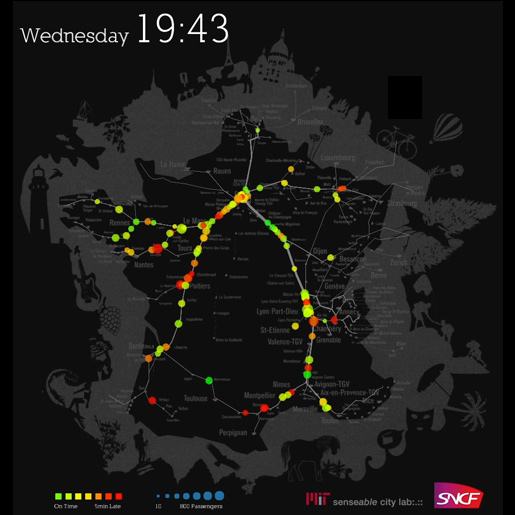
\includegraphics[width=.6\textwidth]{../figuras/trains-of-data.jpg}
  \caption[Visualização baseada no mapa das ferrovias da França]{Posição dos trens às 19:43 na França com uma visualização baseada no mapa
das ferrovias. Fonte: \citet{Senseable2018}.}
  \label{fig:trains-of-data}
\end{figure}

  \item[Visualização baseada em linhas:] visualizações baseadas em linhas são
desenhadas para mostrar a trajetória de objetos, mapas de vias e estradas em
uma região, ou fluxos do tráfego em uma rede de transporte. As trajetórias e
fluxos são representados por linhas ou curvas e são escaladas ou coloridas de
acordo com suas propriedades (i.e. densidade, direção, velocidade).
\citet{Klein2013} apresenta um sistema iterativo para análise do tráfego aéreo
na França. Cada trajetória é representada por uma linha que conecta os pontos
de partida e chegada de cada voo, como pode ser visto na Figura
\ref{fig:air-traffic}.

\begin{figure}[!htb]
  \centering
  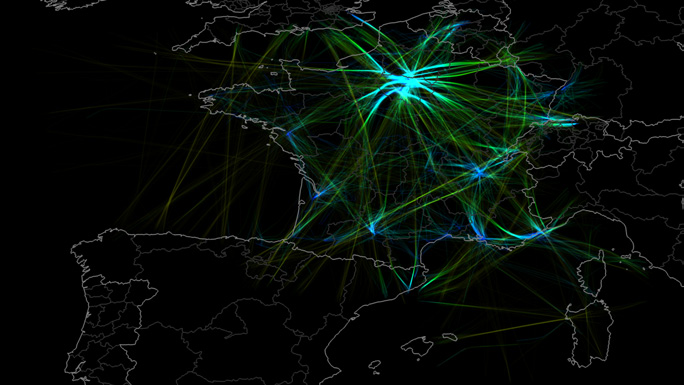
\includegraphics[width=1\textwidth]{../figuras/air-traffic.png}
  \caption[Visualização do tráfego aéreo na França]{Visualização do tráfego aéreo na França. Fonte: \citet{Klein2013}.}
  \label{fig:air-traffic}
\end{figure}

  A representação espacial das linhas pode ainda sofrer transformações
geométricas e topológicas que geram novas abstrações. Por exemplo,
\citet{Tarik2009} mostram uma proposta que transforma as trajetórias de um
leiaute espacial (Figura \ref{fig:viz-espacial}) para um leiaute abstrato
(Figura \ref{fig:viz-abstrata}) para visualizar a movimentação de pessoas
durante a fuga de uma explosão em um escritório.  A abordagem abstrata é usada
para mostrar mais efetivamente os padrões de movimentação de pessoas que se
movem ao mesmo tempo para as mesmas áreas. Na Figura \ref{fig:viz-abstrata} é
possível notar a movimentação de indivíduos antes da explosão (linhas azuis), o
que sugere possíveis suspeitos ou testemunhas do evento.  Além disso, as
informações temporais são difíceis de representar no leiaute espacial, enquanto
no leiaute abstrato o eixo X denomina a sequência do tempo e o eixo Y os locais
no espaço.

\begin{figure}[ht!]
  \centering
  \begin{subfigure}[t]{0.45\textwidth}
    \centering
    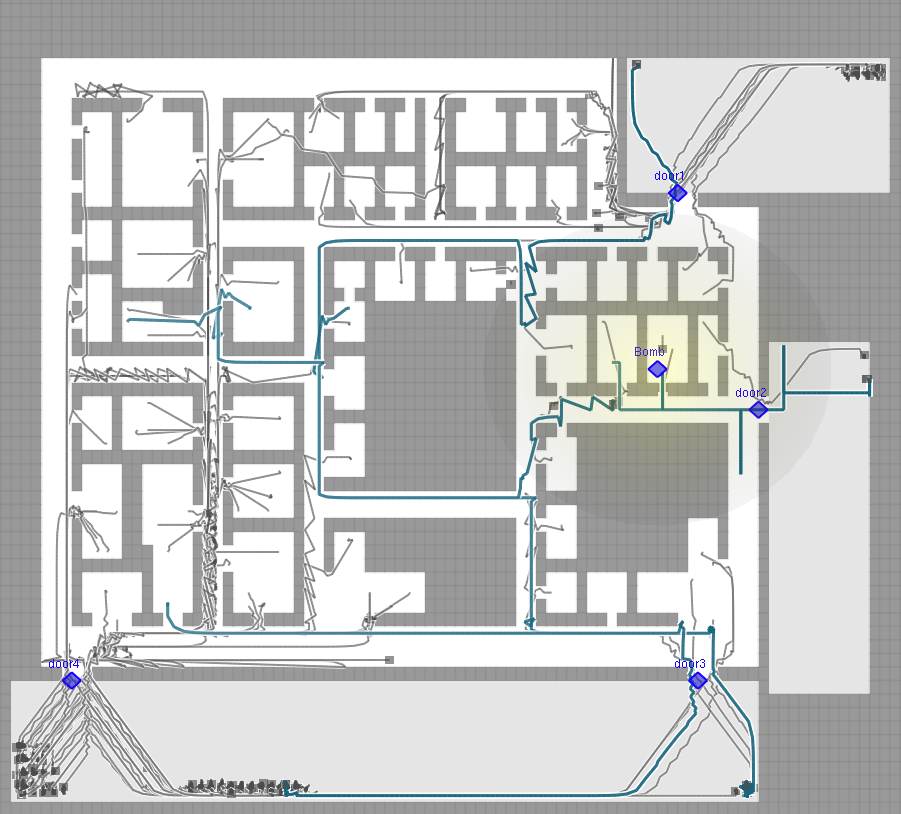
\includegraphics[width=65mm]{../figuras/proximidade-espacial.png}
    \caption{Visualização espacial das trajetórias ao longo do tempo. \label{fig:viz-espacial}}
  \end{subfigure}
  ~
  \begin{subfigure}[t]{0.45\textwidth}
    \centering
    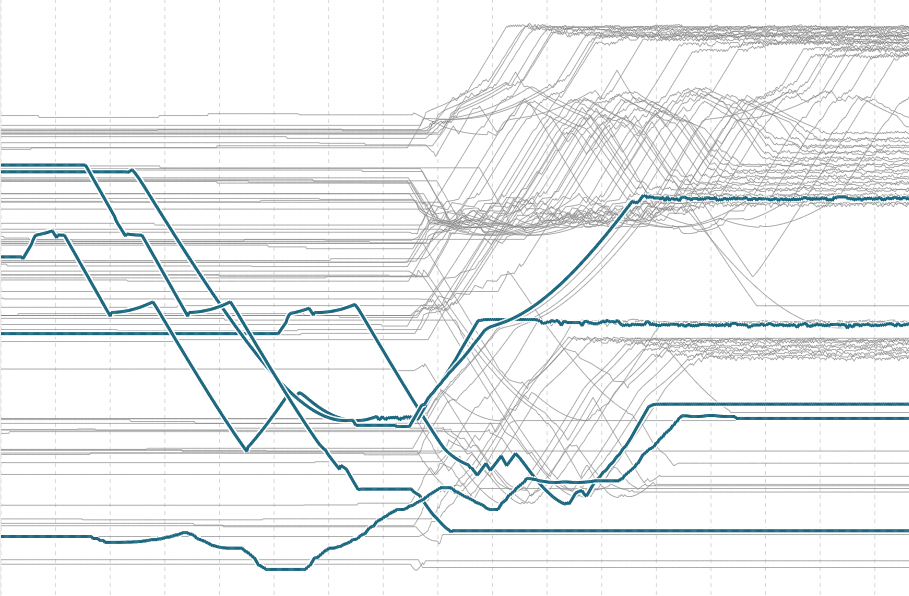
\includegraphics[width=75mm]{../figuras/proximidade-abstrata.png}
    \caption{Visualização abstrata da movimentação ao longo do tempo. \label{fig:viz-abstrata}}
  \end{subfigure}

  \caption[Visualização cartesiana vs abstrata da movimentação de pessoas em um
escritório]{Simulação de uma evacuação de um escritório depois de uma explosão.
(a) Visualização da movimentação da trajetória das pessoas no espaço. (b)
Visualização abstrata, baseada na proximidade.  Fonte: \citet{Tarik2009}.
\label{fig:tarik}}
\end{figure}

  No entanto, a medida que o número de objetos cresce, aumenta também os
problemas de oclusão, o que acaba afetando a estética da visualização e a
obtenção de informações sobre os dados \citep{Zhou2013}. Uma forma de reduzir
a complexidade de análise de um grande conjunto  trajetórias é utilizando
outras formas de abstração dos dados, como uma visualização baseada em regiões.

  \item[Visualização baseada em regiões:] Esse tipo de abstração agrupa fluxos
de deslocamento com origem e destino similares em um nível de macro regiões,
geralmente determinado por divisões administrativas.  \citet{Zeng2013}
apresentam um diagrama em círculos para mostrar padrões de movimentação de
pessoas entre as regiões da cidade. O círculo representa a junção ou conexão
entre as diferentes regiões e o fluxo entre elas. A densidade do fluxo é medido
pela espessura, bem como a direção é destacada dentro do círculo, como é
ilustrado na Figura \ref{fig:interchange-circo}. Apesar de facilitar a
visualização, esse tipo de agregação abre mão das informações individuais de
cada trajetória em favor de uma visão condensada dos fluxos.

\begin{figure}[!htb]
  \centering
  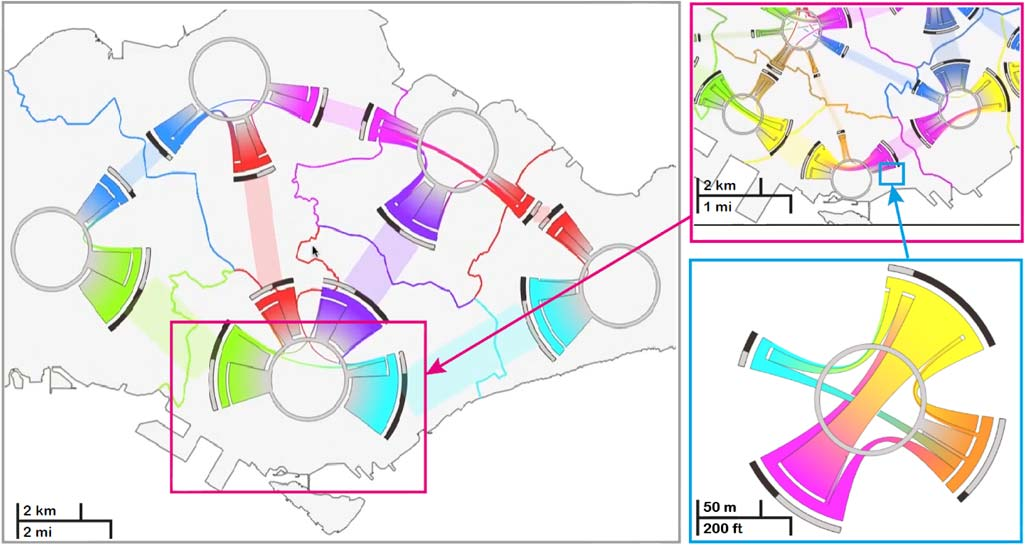
\includegraphics[width=1\textwidth]{../figuras/region-based.png}
  \caption[Exemplo de visualização baseada em regiões do sistema de metrô na França]{Exemplo de visualização baseada em regiões: padrões regionais de movimentação no sistema de metrô na França. Fonte: \citet{Zeng2013}.}
  \label{fig:interchange-circo}
\end{figure}
\end{description}

\section{\emph{Bundling}}
\label{sec:bundling}

  Um grande problema na visualização de grafos e dados de trajetórias é a
oclusão visual à medida que a quantidade de elementos aumenta. Uma pequena
quantidade de dados já começa a apresentar problemas de sobreposição e
cruzamento de arestas, o que dificulta a obtenção de informação sobre os dados.
Uma maneira de contornar esse problema é através de filtros que determinam a
quantidade de itens na visualização. Como consequência do filtro perde-se a
visão global de todos os itens ao mesmo tempo, o que pode ser necessário para a
identificação das correlações e padrões entre eles. Uma outra abordagem é o uso
de agregações que geram novas abstrações dos dados. Na seção anterior mostramos
como o agrupamento em regiões projetado sobre um diagrama circular simplifica a
visualização das trajetórias entre as áreas da cidade.

 Uma solução que tem sido amplamente utilizada em várias pesquisas de
visualização de dados de tráfego é o uso de uma técnica chamada
\emph{bundling}. A técnica ajuda a simplificar o desenho da visualização
através da agregação espacial das arestas em conjuntos chamados
\emph{bundles}, que funcionam de forma similar a algoritmos de clusterização. Os \emph{bundles} são
definidos como um grupo de arestas similares, compatíveis o suficiente para
serem representadas por um corpo único e compacto \citep{Lhuillier2017}. A
compatibilidade é calculada a partir de uma função de similaridade usada para
determinar quais arestas devem fazem parte do mesmo agrupamento.
Imaginando então algumas viagens no trânsito, podemos agrupá-las pela sua
região de origem, destino, distância percorrida, direção ou até mesmo o meio de
transporte utilizado.  Dessa forma, o número de \emph{bundles} é ligeiramente
inferior ao número de trajetórias a serem desenhadas, ficando mais simples
compreender e visualizar a estrutura global, padrões e tendências entre grupos
de trajetórias que ligam áreas fortemente relacionadas \citep{Zhou2013}.  A
Figura \ref{fig:bundling-hierarquico} mostra o uso de uma técnica de
\emph{bundling} para visualização da hierarquia de módulos e arquivos de um
software onde as arestas mostram suas relações de dependência. A ligação
acontece quando um módulo acessa atributos e/ou funções definidos em outras partes
do software.

\begin{figure}[!htb]
  \centering
  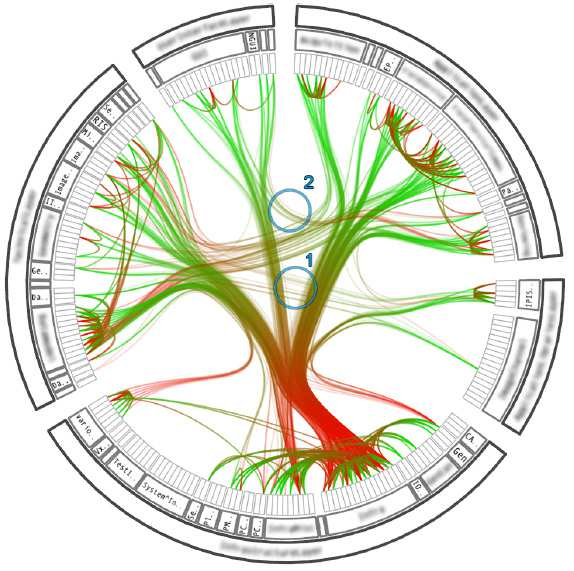
\includegraphics[width=.5\textwidth]{../figuras/hbundling.png}
  \caption[Bundling hierárquico na visualização de dados de software]{Bundling hierárquico na visualização de dados de software. As cores mapeiam
o sentido do acesso, verde é a origem, vermelho é o alvo. Fonte: \citep{Holten2006}.}
  \label{fig:bundling-hierarquico}
\end{figure}

\subsection{Modelos de \emph{Bundling}}

  O cálculo de um \emph{bundle} não possui uma definição precisa, e por isso há
uma grande variedade de algoritmos e abordagens para modelar problemas de
agrupamento de arestas com \emph{bundling}, que podem variar significativamente
de um para outro em questões de complexidade e aplicação dos algoritmos
\citep{Zhou2013}.  \emph{Force-directed edge bundling} (FDEB), apresentado em
\citet{Holten2009}, cria \emph{bundles} através da atração entre pontos de
controle colocados ao longo das arestas e é considerado um modelo baseado em
custo, já que tenta minimizar o valor de uma função de custo que representa a
força de atração entre as arestas.  \emph{Hierarchical Edge Bundling} (HEB)
agrupa as arestas baseadas na estrutura hierárquica do grafo para o cálculo dos
\emph{bundles} e por isso é considerado um modelo geométrico \citep{Holten2006}. Outra
classificação são os modelos baseados em imagem, como \emph{Skeleton-based edge
bundling} (SBEB) e \emph{Kernel Density Estimation-based Edge Bundling}
(KDEEB), que surgiram mais recentemente. Eles utilizam algoritmos de
clusterização para extrair a estrutura geral do grafo para então calcularem os
\emph{bundles}. O algoritmo SBED utiliza o esqueleto do grafo como guias para
criar \emph{bundles} com muitas ramificações \citep{Ersoy2011}, enquanto o
KDEEB utiliza um mapa de densidade do grafo para extrair sua estrutura no
espaço da imagem \citep{Hurter2012}. A Figura \ref{fig:subfigures} dá um
exemplo da variedade de possíveis saídas geradas por diferentes algoritmos de
\emph{bundling} (FDEB, SDEB e KDEEB) aplicados nos mesmos dados.  Nesse exemplo
são usados dados de uma semana do tráfego aéreo sobre os EUA.

\begin{figure}[!htb]
  \centering
  \begin{subfigure}{0.6\textwidth}
    \centering
    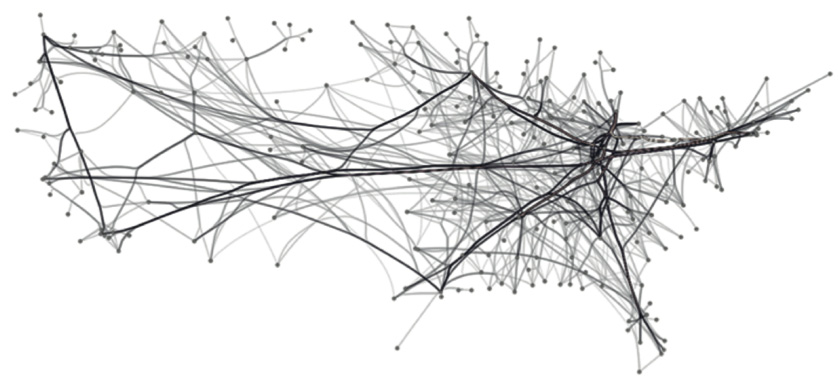
\includegraphics[width=1\textwidth]{../figuras/FDEB.png}
    \caption{FDEB}
    \label{fig:FDEB}
  \end{subfigure}

  \begin{subfigure}{0.6\textwidth}
    \centering
    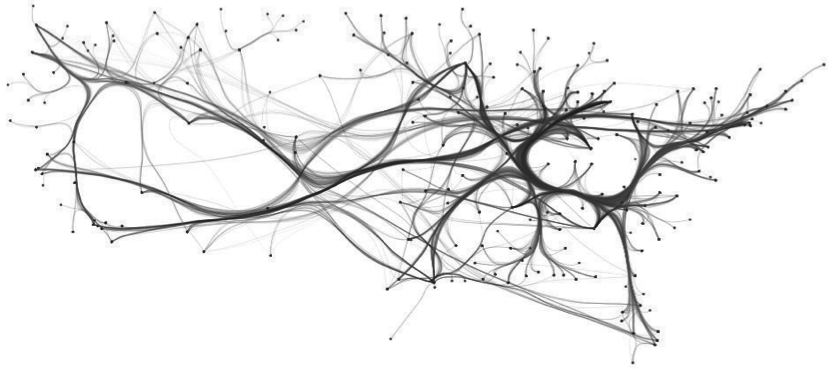
\includegraphics[width=1\textwidth]{../figuras/SBEB.png}
    \caption{SBEB}
    \label{fig:SBEB}
  \end{subfigure}

  \begin{subfigure}{0.6\textwidth}
    \centering
    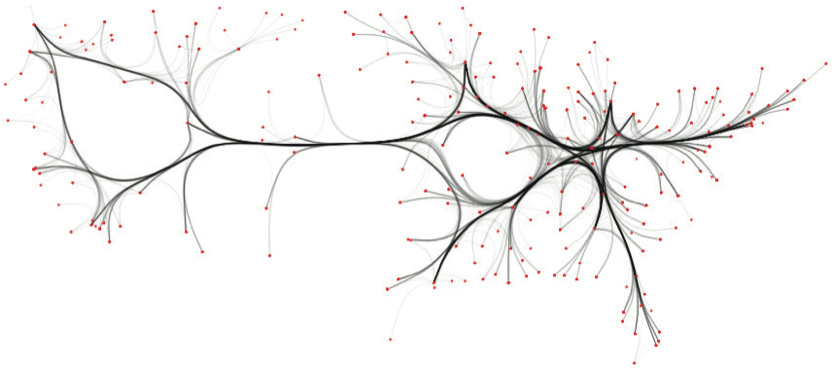
\includegraphics[width=1\textwidth]{../figuras/KDEEB.png}
    \caption{KDEEB}
    \label{fig:KDEEB}
  \end{subfigure}
  \caption[Diferentes algoritmos de \emph{bundling} aplicadas nos mesmos dados]{Diferentes algoritmos de \emph{bundling} aplicadas em dados do tráfego aéreo dos EUA - 235 nós, 2099 arestas. Fonte: \citep{Klein2013}.}
  \label{fig:subfigures}
\end{figure}

  A escolha do modelo geralmente parte da observação e experiências de
aplicação em problemas semelhantes, já que conhecer e testar diferentes
abordagens e suas variações não é uma tarefa simples. Por isso,
\citet{Lhuillier2017} recentemente propôs uma nova taxonomia para os modelos e
algoritmos de \emph{bundling} dividindo-os com base no tipo de dados em que se deseja
aplicar a técnica. Eles justificaram que desta forma pesquisadores e usuários
da técnica pudessem focar no seu contexto de aplicação e não em detalhes
específicos de implementação algorítmica. Seu estudo dividiu os modelos
existentes inicialmente em dois grupos, conforme o tipo de dados, grafos ou
trajetórias. Então, mais detalhes sobre a direção (direcionado ou não),
dimensão (2D ou 3D) e dependência do tempo (dinâmico ou estático) refinam a
divisão dentro da sua taxonomia.


\begin{figure}[!htb]
  \centering
  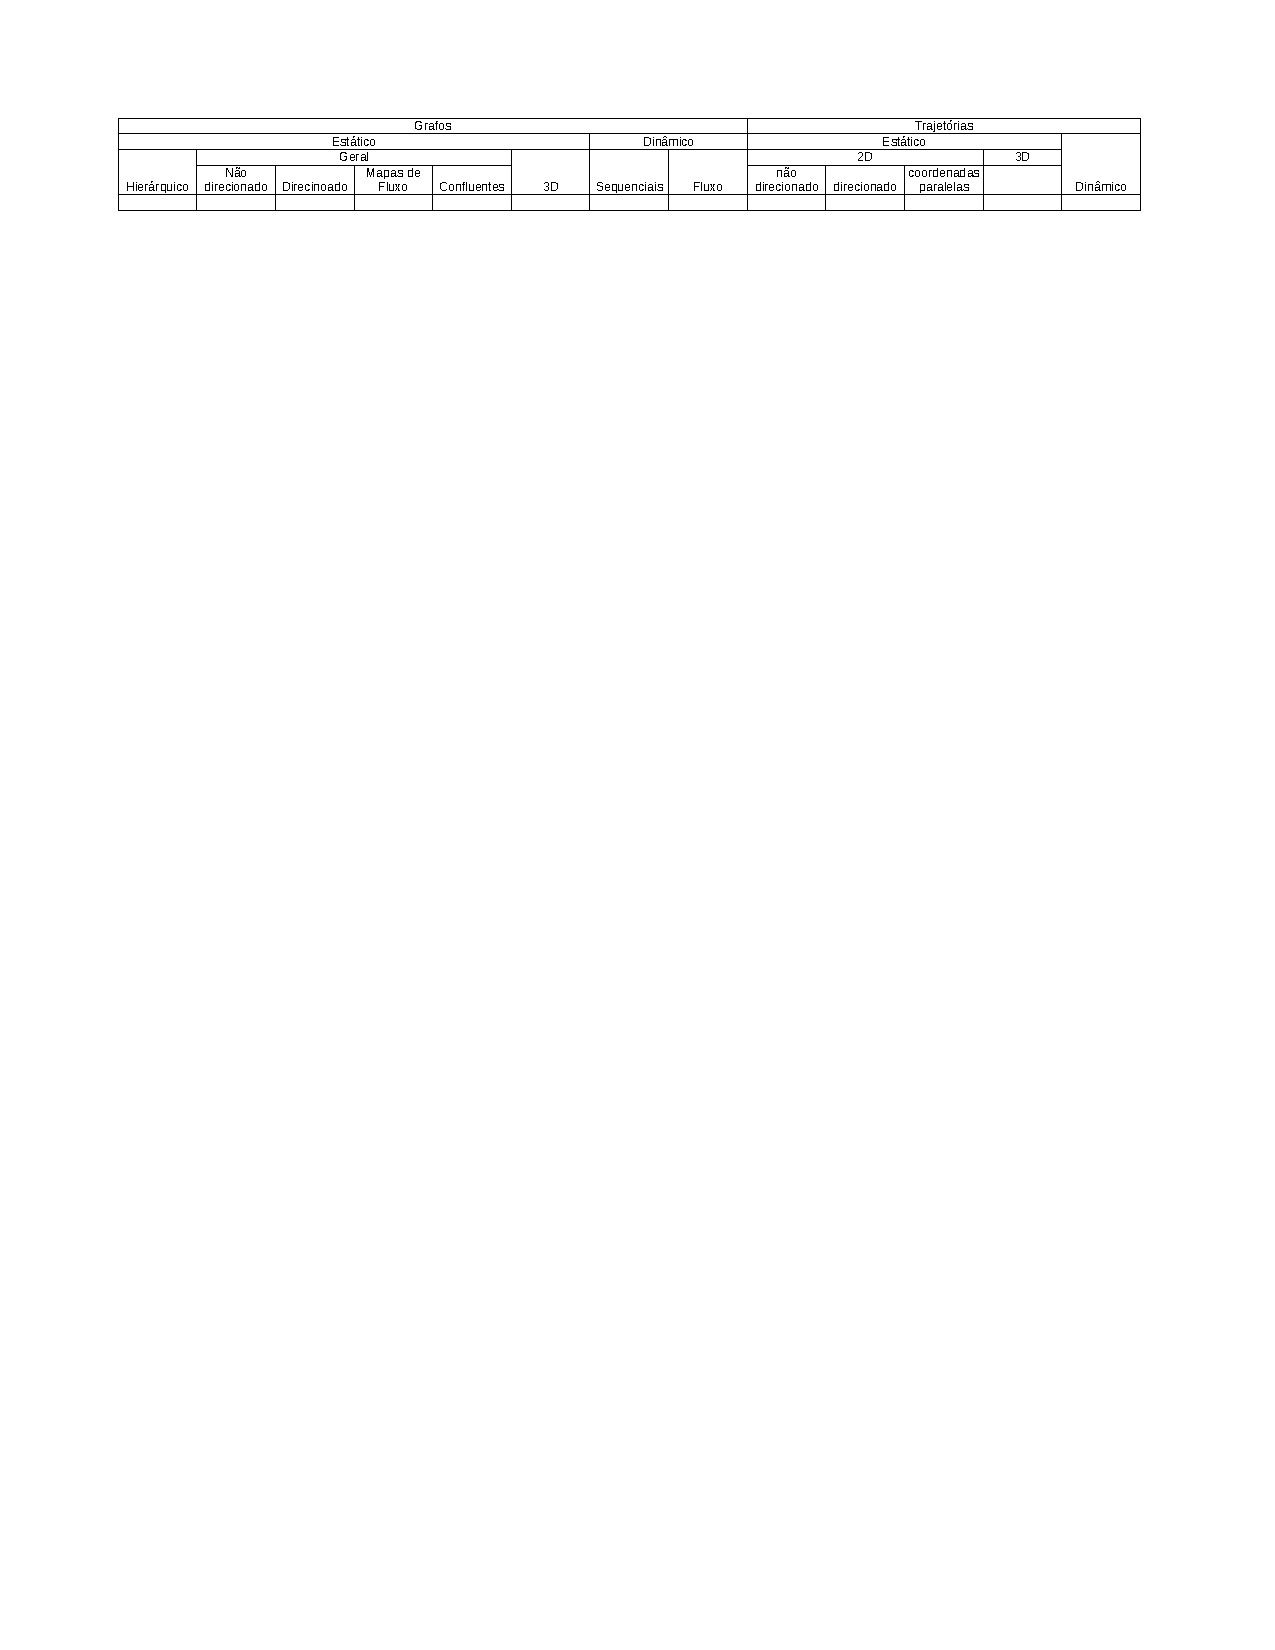
\includegraphics[width=\textwidth]{../figuras/estado-da-arte.pdf}
  \caption[Taxonomia dos métodos de \emph{bundling} baseado no tipo de dado]{Taxonomia dos métodos de \emph{bundling} baseado no tipo de dado. Fonte: \citet{Lhuillier2017}}
  \label{table:bundling-methods}
\end{figure}


Podemos então seguir a taxonomia para selecionar uma método de
\emph{bundling} que seja mais adequado para a análise de fluxos no trânsito da
cidade. \emph{Attribute-Driven Edge Bundling} (ADEB) é um algoritmo que segue um
modelo baseado em imagem e é apresentado dentro desta taxonomia como um das
opções para a análise de dados de trajetórias direcionadas. Discutimos na
próxima seção as características desse modelo e como podemos nos beneficiar
dele em nosso estudo.

\subsection{Modelo Baseado em Imagem}
\label{sec:modelo-imagem}

  Uma das etapas do \emph{bundling} é a identificação das trajetórias
similares, que requerem que cada uma delas seja comparada a todos os outras
para descobrir quais são as mais próximas, afim de agrupá-las em
\emph{bundles}.  Esse cálculo, no entanto, é bastante custoso e pode demorar
minutos em cenários com milhares de trajetórias.

\emph{Kernel Density Estimation Edge Bundling} (KDEEB) é um algoritmo proposto
por \citet{Hurter2012}. Eles observaram que ao aplicar uma operação de \emph{bundling} $B$ qualquer sobre um
grafo $G$, o resultado são áreas de maior densidade (dentro dos \emph{bundles})
e áreas de menor densidade fora deles, em comparação ao grafo original. Assim,
essa operação \emph{bundling} $B$ pode ser moldada em função de uma operação
sobre a densidade dos pontos do grafo, similar ao que faz o algoritmo de
clusterização \emph{Mean Shift} \citep{Comaniciu2012}. A partir disso, a heurística
desse algoritmo de \emph{bundling} consiste em computar repetidamente o
gradiente dos pontos em relação à uma função de densidade, e então movendo-os
para regiões mais densas apontadas pelo gradiente. O maior benefício do método
é sua implementação paralela com o uso do poder computacional de placas
gráficas (GPUs), o que levou a ganhos de desempenho de uma ordem de magnitude
em relação a métodos anteriores. KDEEB representou uma abertura para uma área
chamada \emph{image-based bundling}, ou métodos baseados em imagem, onde $B$ é
implementado via operações de processamento de imagem, diferentemente de
métodos puramente geométricos existentes até então. O algoritmo consiste nos
seguintes passos:

\begin{enumerate}
  \item Converte o grafo $G$ em um mapa de densidade usando uma função de
densidade. A função utilizada é um estimador baseado em núcleos, geralmente um
estimador Gaussiano ou Epanechnikov.

  \item Computar o gradiente da função de densidade para cada ponto/nó do
grafo. O cálculo do gradiente indica a direção onde há maior quantidade
de nós/arestas aglomeradas no grafo.

  \item Mover os nós na direção do gradiente (áreas mais densas). Essa etapa é
suavizada movendo-se os nós pela norma do gradiente, ou seja, em apenas uma unidade
a cada iteração. Isso evita que as arestas dêem grandes saltos.

  \item Corrigir distorções causadas pela movimentação dos nós com filtro
Laplaciano (opcional).  O passo anterior pode causar pequenas distorções, como
por exemplo, a sobreposição de nós. Esta é uma forma de se corrigir essas
distorções sem que se perca a estrutura geral do grafo.

  Repetir a partir do passo 1 até a convergência do algoritmo, o que leva cerca de 8..10
iterações.
\end{enumerate}

%\citet{Hurter2012} apresentam ainda uma maneira para limitar os \emph{bundles}
%com relação a obstáculos presentes no caminho das arestas. Um obstáculo
%qualquer, representado por seus limites espaciais pode ser contornado
%alterando-se a função de densidade, que sofre uma degradação dentro da área
%geométrica do obstáculo. Com isso, o gradiente age como uma força de repulsão
%das arestas que cruzam o obstáculo e faz com que as arestas sejam movidas
%na direção pra fora de suas bordas.

  {\emph{Attribute-Driven Edge Bundling} (ADEEB) é uma extensão do algoritmo
KDEEB, proposta por \citet{ZegarraFlores2016}, e que permite a separação das
arestas conforme sua direção. Essa informação é obtida percorrendo cada aresta
a partir do ponto de origem até o destino e calculando para cada uma delas um
vetor unitário que aponta a sua direção, que é mapeado para o
ângulo desse mesmo vetor. Então, cria-se um mapa de densidade direcionado, onde são
consideradas apenas as arestas que vão na mesma direção (mesmo ângulo). Esse
algoritmo herda todos os benefícios de desempenho e robustez apresentados pelo
KDEEB, o que o faz um método adequado para a análise do tráfego de veículos no
trânsito da cidade.

\subsection{\emph{Bundling} em Dados Dinâmicos}

  Um grafo dinâmico é aquele no qual seus nós e arestas são dependentes do
tempo, ou seja, a cada momento \emph{t}, existe um grafo G(t) diferente a ser
explorado. Nesse contexto, dois diferentes tipos de grafos dinâmicos podem ser
considerados, grafos sequenciais e grafos de fluxo \citep{Hurter2013}. Um
grafo sequencial consiste em um conjunto de grafos $G^i = (V^i, E^i)$, onde
cada grafo $G^i$ é como um retrato no momento $i$ de um sistema que é
dependente do tempo. Grafos de fluxo, por outro lado, são definidos como um
conjunto de vértices $V$ e arestas $E$, onde as arestas são definidas pelo seu
tempo de vida e nós. Grafos de fluxo não possuem uma sequência pré-definida e
são tipicamente obtidos de fontes de dados online.

  O uso de \emph{bundling} nesse cenário é similar a outros métodos de
visualização de grafos dinâmicos. Para grafos sequenciais o \emph{bundling} é
aplicado a cada grafo $G^i$ de maneira estática. Já em grafos de fluxo, os
dados são divididos em janelas de tempo e o algoritmo é aplicado em cada
intervalo $\Delta t$, que podem ser colocados lado a lado para comparação em
uma técnica conhecida como \emph{small multiples}. Uma outra maneira de se
visualizar a dinâmica é com o uso de animações, como mostram
\citet{Hurter2014}. A vantagem desse método sobre o anterior é que ele se
adequa melhor à análise de longas séries temporais.

\section{Simulação do Tráfego de Veículos}

  O crescimento da população nas cidades ao redor do mundo trouxe também vários
desafios de gestão e controle do trânsito, especialmente em grandes cidades,
que precisam lidar com vários problemas de congestionamentos, acidentes,
poluição, controle do transporte público, entre outros. Uma maneira alternativa
para estudar e solucionar esses problemas é através do uso de ferramentas de
simulação. Essas ferramentas permitem criar cenários do tráfego de veículos e
ajudam nos estudos sobre seu comportamento e na elaboração de soluções para
serem aplicadas por gestores das cidades. Recentemente, novas ferramentas de
simulação com foco em escalabilidade foram desenvolvidas, permitindo testes e
experimentos em escala real de uma grande cidade, com milhões de veículos. O
InterSCSimulator é uma destas ferramentas e o detalhamos a seguir.

\subsection{InterSCSimulator}
\label{sec:interscsimulator}

\citet{mabs2017} apresentam o InterSCSimulator, uma ferramenta de código livre,
capaz de executar simulações com mais de 4 milhões de veículos em uma grande
metrópole.  As simulações são feita em escala mesoscópica. Isso significa que
ela segue um modelo onde cada veículo do trânsito é simulado individualmente. O
simulador calcula para cada um deles as ações de movimentação durante sua
viagem.

\subsubsection{Componentes do InterSCSimulator}

  O simulador possui quatro componentes principais: o \textbf{cenário}, que
recebe os arquivos de entrada e cria o grafo da cidade e os primeiros veículos;
\textbf{o motor de simulação}, que executa os algoritmos e modelos da simulação
para gerar os arquivos com os resultados; um componente de
\textbf{visualização do mapa}, que recebe o arquivo de saída com os resultados
e gera uma visualização da simulação baseada em pontos; e finalmente um
componente de \textbf{visualização de gráficos} que gera uma série de gráficos
com informações sobre o cenário simulado, como velocidade média dos veículos ao
longo do tempo e outros. A Figura \ref{fig:interscsimulator} ilustra a
interação entre os componentes e os arquivos de entrada e saída.

\begin{figure}[!htb]
  \centering
  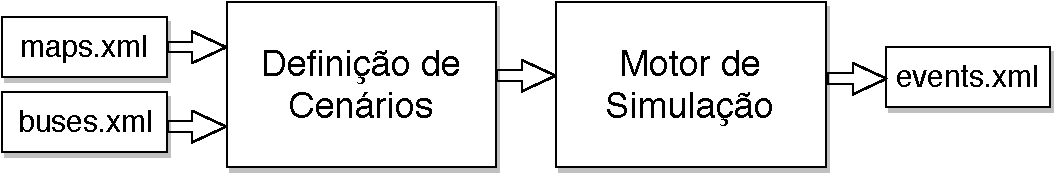
\includegraphics[width=\textwidth]{../figuras/arquitetura-simulador.pdf}
  \caption[Componentes do InterSCSimulator]{Componentes do InterSCSimulator. \label{fig:interscsimulator}}
\end{figure}

  O simulador utiliza dois arquivos principais de entrada para definição do
cenário, são eles map.xml e trips.xml. O primeiro contém a descrição da rede
rodoviária da cidade e é construído com dados obtidos de serviços como Open
Street Maps (OSM)\footnote{\rurl{openstreetmap.org}}. O arquivo é composto por
nós e links, que representam cruzamentos e ruas, respectivamente. A Listagem
\ref{map.xml} mostra um exemplo de um arquivo map.xml com 3 nós e 3 links. Um
usuário da simulação pode ainda fazer alterações nesse arquivo para alterar o
mapa da cidade para atender a um novo cenário, como por exemplo, remover os nós
e links de uma rua conhecida para simular o bloqueio causado por um acidente.
Utilizaremos desse mecanismo para estudar diferentes cenários do trânsito.

\begin{lstlisting}[style=myxml, caption={Exemplo de arquivo map.xml que define a rede rodoviária da cidade. Fonte: \citet{mabs2017}}, label=map.xml]
<network>
  <nodes>
   <node id ="1" x="-46.65805" y="-23.58162"/>
   <node id ="2" x="-46.65828" y="-23.58342"/>
   <node id ="3" x="-46.65228" y="-23.59341"/>
  </nodes>
  <links>
    <link id="35985" from="1" to="2" length="100" free speed="40"/>
    <link id="35985" from="2" to="3" length="200" free speed="40"/>
    <link id="35985" from="3" to="1" length="80"  free speed="50"/>
  </links>
</network>
\end{lstlisting}

  O segundo arquivo de entrada, \emph{trips.xml}, descreve todas as viagens que
devem ser simuladas. Cada viagem deve informar os nós de origem e destino e o
horário da simulação em que ela será iniciada, como pode ser visto na Listagem
\ref{trips.xml}. O caminho entre a origem e o destino pode ainda ser fixada
previamente nesse arquivo ou pode ser calculado pelo simulador, o qual fica
responsável por determinar a rota a ser seguida. Um aspecto interessante é que
se quisermos duplicar o tamanho da simulação, podemos fazer isso simplesmente
duplicando as linhas desse arquivo.

\begin{lstlisting}[style=myxml, caption={Exemplo de arquivo trips.xml que define a rede rodoviária da cidade. Fonte: \citet{mabs2017}}, label=trips.xml]

<scsimulator_matrix>
  <trip origin="247951669" destination="60641382"
    type="car" start_time="28801"/>
  <trip origin="60641382" destination="247951669"
    type="car" start_time="63001"/>
  <trip origin="4511105625" destination="2109902387"
    type="car" start_time="16201"/>
  <trip origin="247951669" destination="60641382"
    type="car" start_time="54001"/>
  <trip origin="246650787" destination="247951670"
    type="car" start_time="54001"/>
  <trip origin="247951670" destination="246650787"
    type="car" start_time="66601"/>
  <trip origin="246650787" destination="60641382"
    type="bus" start_time="54001"/>
</scsimulator_matrix>
\end{lstlisting}

  Cada veículo (carro ou ônibus) definido no arquivo \emph{trips.xml} é um
elemento independente dentro da simulação. Eles percorrem seu trajeto do nó de
origem até o nó de destino seguindo a rede rodoviária da cidade definida no
arquivo \emph{map.xml}.  Cada veículo possui quatro estados dentro da
simulação: \emph{Start}, quando o tempo da simulação atinge o tempo de início
do veículo; \emph{Move}, quando a simulação atinge o tempo do próximo movimento
do veículo; \emph{Wait}, quando o veículo tem que esperar até o próximo
movimento; e \emph{Finish}, quando o veículo chega ao seu destino. Os estados
representam eventos ocorridos dentro da simulação, que são registrados no
arquivo de saída \emph{events.xml}. A Listagem \ref{events.xml} mostra parte de
um arquivo de saída gerado durante uma simulação. É possível ver os eventos de
\emph{start\_trip}, \emph{move} e \emph{finish\_trip} para dois veículos com os
identificadores $2121$ e $2223$.  É importante notar também o atributo
\emph{time}, que indica o tempo de ocorrência do evento dentro da simulação.
Esse atributo  é contabilizado em segundos. Na simulação de um dia do trânsito,
por exemplo, temos então 86400 segundos, correspondentes às 24 horas do dia.

\begin{lstlisting}[style=XML, caption={Exemplo de arquivo de saída events.xml com os eventos da simulação. Fonte: \citet{mabs2017}}, label=events.xml]

<events version="1.0">
  <event time="4" type="start_trip" vehicle="2121" link="5243" />
  <event time="4" type="start_trip" vehicle="2223" link="1002" />
  <event time="11" type="move" vehicle="2223" link="4005" />
  <event time="31" type="move" vehicle="2121" link="4005" />
  <event time="38" type="move" vehicle="2223" link="2007" />
  <event time="52" type="finish_trip" vehicle="2121" link="4005" />
  <event time="52" type="finish_trip" vehicle="2223" link="5243" />
</events>
\end{lstlisting}

  A partir desse arquivo de saída e do mapa da cidade é possível montar o o
rastro de mobilidade dos veículos ao longo do tempo, recuperando as posições de
latitude e longitude dos \emph{links} sobre o qual eles se movimentam, como
mostra a Tabela \ref{table:rastro}. O rastro de um veículo da simulação pode
ser visto na Figura \ref{fig:rastro}. O ponto verde indica a origem na cor
preta está marcado o destino. Já os pontos vermelhos marcam cada evento de
movimentação que ele fez dentro da simulação.

\begin{table}[!htb]
\centering
\begin{tabular}{|c|c|c|c|c|}
\hline
\textbf{Horário} & \textbf{Ação} & \textbf{ID} & \textbf{Latitude} & \textbf{Longitude} \\
\hline
25 & start & 4858\_52 & -23.624235 & -46.648388 \\
27 & start & 4858\_73 & -23.624235 & -46.648388 \\
27 & start & 94\_17 & -23.535976 & -46.63561    \\
31 & move & 4858\_52 & -23.624077 & -46.648453 \\
33 & move & 4858\_73 & -23.624077 & -46.648453 \\
35 & start & 8394\_43 & -23.561275 & -46.695423 \\
\hline
\end{tabular}
\caption{Tabela com o rastro do tráfego montado a partir do arquivo de saída e o mapa da cidade. \label{table:rastro}}
\end{table}

\begin{figure}[!htb]
  \centering
  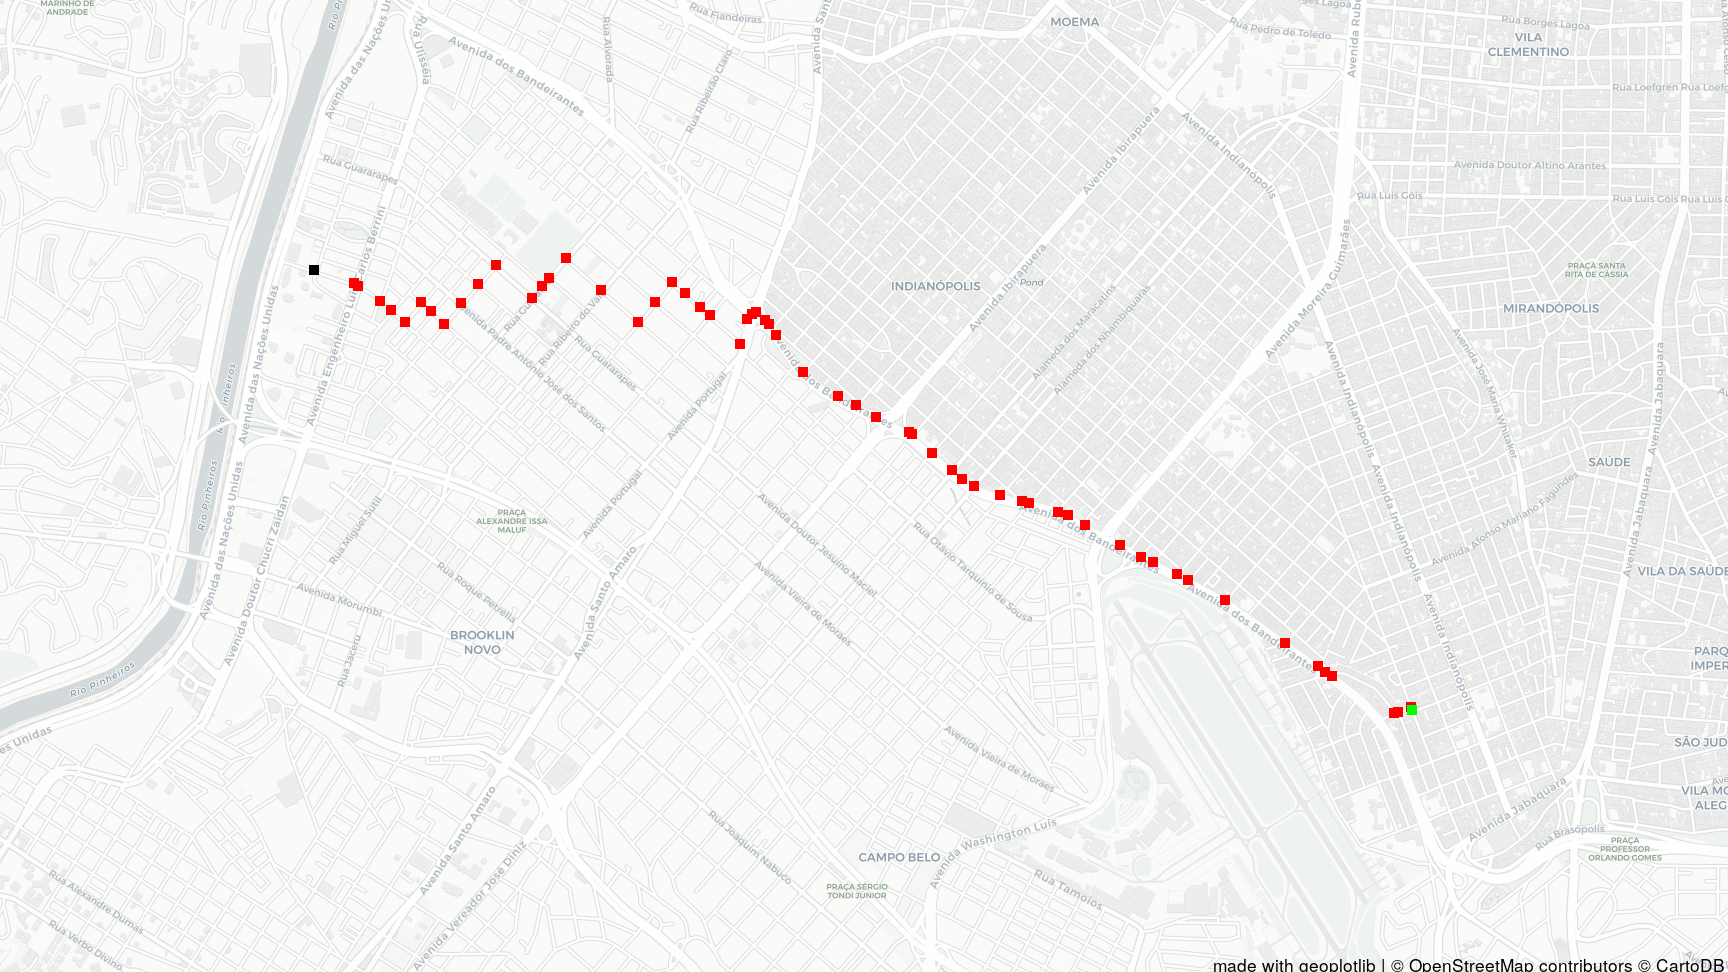
\includegraphics[width=\textwidth]{../figuras/pontos.png}
  \caption{Visualização dos pontos da trajetória do veículo com ID 4858\_52. \label{fig:rastro}}
\end{figure}

Já a Figura \ref{fig:simulated-traffic} mostra uma simples visualização em linhas
de um conjunto de trajetórias do tráfego simulado. Os dados são resultado
da pesquisa de \citet{santana2018courb}, que criaram uma simulação com milhares
de veículos e disponibilizaram os arquivos com os resultados. Utilizamos dados
no intervalo de 1 hora do trânsito filtrando pontos que estivessem entre os
intervalos de tempo $21600$ e $25200$, o que corresponde ao horário entre 6 e 7
da manhã. Note que há bastante oclusão, sendo também impossível distinguir
quais origens vão para quais destinos ou a quantidade de veículos nas vias.

\begin{figure}[!htb]
  \centering
  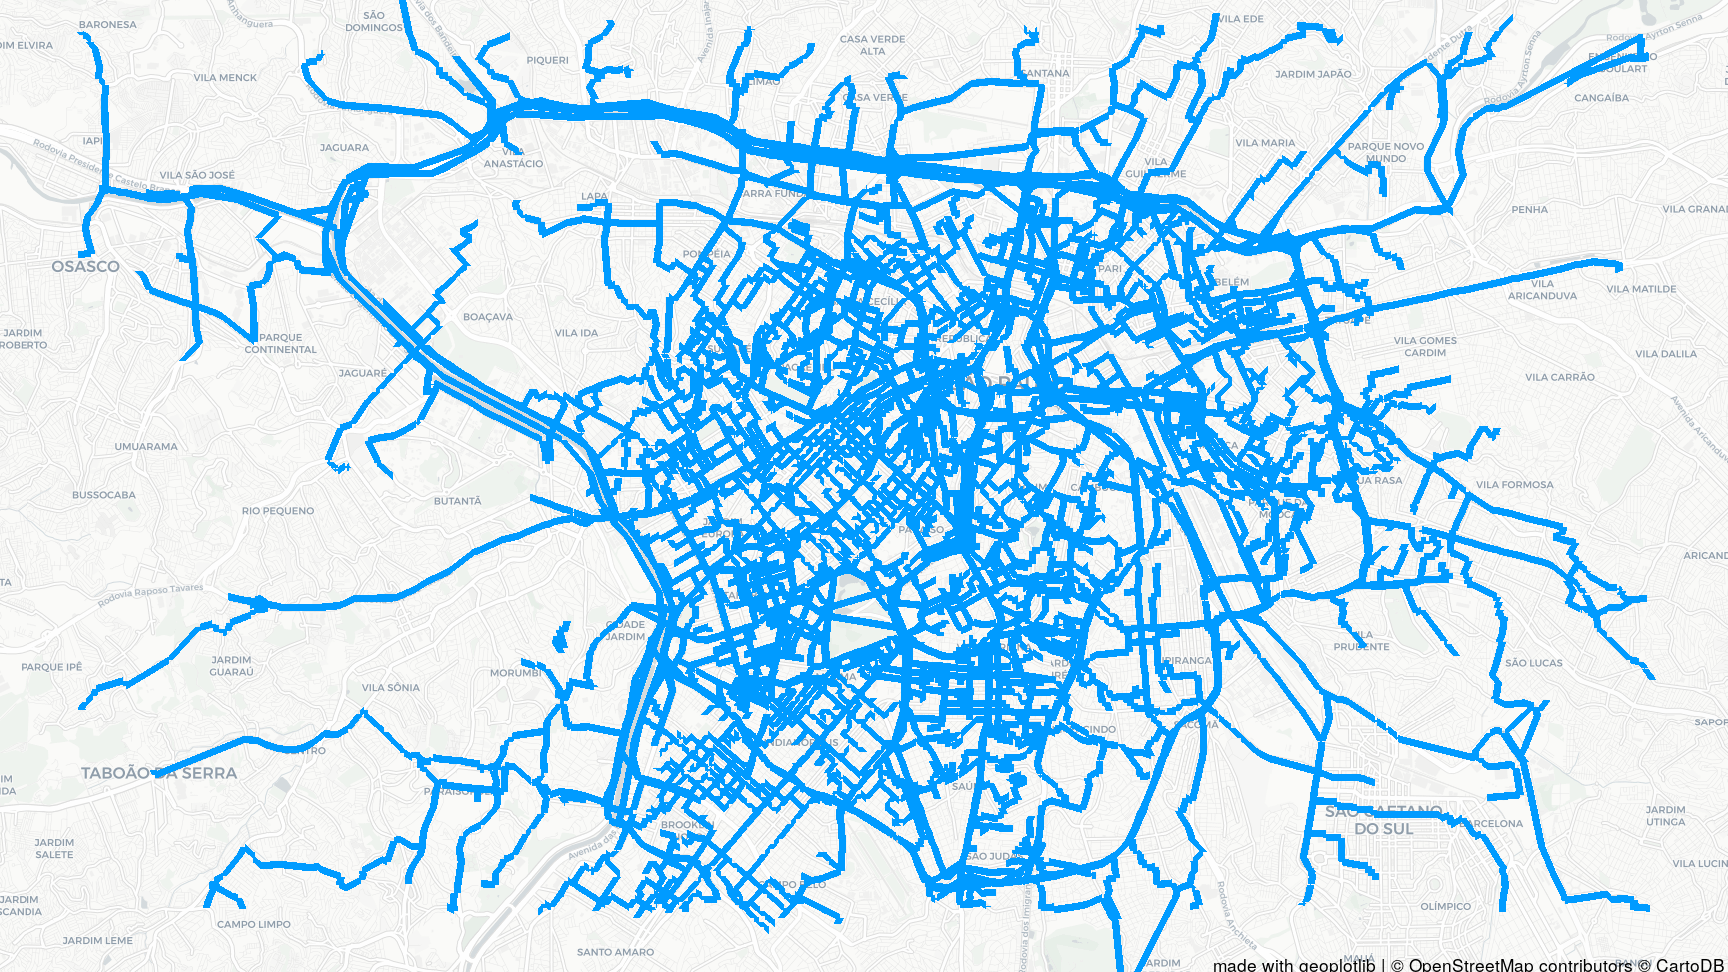
\includegraphics[width=1\textwidth]{../figuras/trafego-ocluso.png}
  \caption{Simulação do tráfego entre 6 e 7 da manhã.}
  \label{fig:simulated-traffic}
\end{figure}

  Os conceitos apresentados montaram de base para a nossa proposta de
visualização dos dados do tráfego de veículos no trânsito. Inclui-se no
processo de formulação da proposta a definição do tipo de visualização que
iremos utilizar, domínio sobre os dados do trânsito e suas propriedades
espaciais e temporais, para posteriormente chegarmos a uma análise dos fluxos
de origem e destino em diferentes níveis de detalhe a partir de um modelo de
\emph{bundling}, propondo também maneiras de destacar essas propriedades dentro
da visualização. No próximo capítulo apresentamos em detalhes a nossa proposta.
